To evaluate the validity of the hypothesis, a typical software engineering process involving an initial \emph{analysis} phase, followed by several \emph{design}, \emph{implementation} and \emph{testing} iterations has been followed. A graphical overview of the process appears in Figure \ref{fig:ResearchMethodology}. This section provides an overview of the main phases of the process.

\begin{figure}
	\centering
		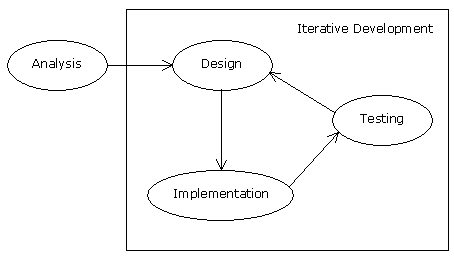
\includegraphics{images/ResearchMethodology}
	\caption{Overview of the research methodology}
	\label{fig:ResearchMethodology}
\end{figure}

\subsection{Analysis}

In the analysis phase, the most widely used metamodelling architectures that enable engineers to define modelling languages and models, and the the most common model management tasks were identified. For each model management task, the state-of-the-art approaches in terms of supporting languages and tools were reviewed in order to identify their advantages and shortcomings. Through the analysis, a number of research challenges have been identified that have motivated the hypothesis and objectives of the thesis.

\subsection{Iterative Design and Implementation}

Following the analysis phase, a conceptual architecture has been conceived to investigate the hypothesis. This conceptual architecture has been refined into a technical design which in turn has guided the construction of the reference implementation.
 
In the first phase of design, infrastructure was designed based on the findings of the analysis. Following this, languages for previously unsupported tasks (model comparison and merging) were built atop the infrastructure. Through the process of building these first task-specific languages, the design and implementation of the infrastructure have been progressively improved and become more flexible in order to accommodate the needs of the different tasks. Latterly, languages for model-to-model transformation, model validation and in-place model transformation were designed and implemented. 

Finally, a workflow mechanism was designed and a prototype was implemented to enable orchestration and coordination of tasks implemented using different task-specific language of the platform.

\subsection{Iterative Testing}

Throughout the design and implementation iterations, several case studies have been used to assess the quality and usefulness of the proposed approach and the correctness of the reference implementation. Also significant feedback has been provided by the academic peers who have, to date, reviewed 18 papers on several core aspects of the design of the platform and the languages that built atop it, and by external users who have been using the reference implementation. Errors and omissions identified during testing iterations were provided as input to further design and implementation cycles.